\documentclass{article}
\usepackage[utf8]{inputenc}
\usepackage{hyperref}
\usepackage{graphicx}
\usepackage{float}
\usepackage{amsmath}
\usepackage{amssymb}
\usepackage{color}
\usepackage[toc,page]{appendix}
\usepackage{booktabs}
\usepackage{longtable}
\usepackage[nottoc,numbib]{tocbibind}
\usepackage{subcaption}
\usepackage{multirow}
\usepackage[table,xcdraw]{xcolor}

\setlength{\textwidth}{15cm}
\setlength{\oddsidemargin}{0in}   %

\title{[IC] Relatório Parcial}
\author{Pedro Henrique Barbosa de Almeida}
\date{January 2019}

\renewcommand{\labelenumii}{\theenumii}
\renewcommand{\theenumii}{\theenumi.\arabic{enumii}.}
\renewcommand{\contentsname}{Sumário}
\renewcommand{\refname}{Referências}
\renewcommand{\appendixpagename}{Apêndices}
\renewcommand{\appendixtocname}{Apêndices}
\renewcommand{\listfigurename}{Lista de figuras}
\renewcommand{\listtablename}{Lista de tabelas}
\renewcommand{\figurename}{Figura}
\renewcommand{\tablename}{Tabela}


\graphicspath{ {imgs/} }

\begin{document}
	
	\thispagestyle{empty}
	
	
	\begin{center}
		{\bf \Large Relatório Final}
		
		MAC0215 - Atividade Curricular em Pesquisa
	\end{center}
	
	\bigskip
	\begin{center}
		{\bf \LARGE Aprendizado de transformações de imagens via classificação de  microrregiões}
		
		\bigskip
		\bigskip
		{\large Pedro Henrique Barbosa de Almeida} \\
		{N. USP 10258793} \\
		{\bf Estudante}
		
		\bigskip
		\bigskip
		{\large Nina S. T. Hirata}\\ 
		Contato: nina@ime.usp.br \\
		{\bf Orientadora}
		
		\bigskip
		\bigskip
		\bigskip
		\bigskip
		
		\bigskip
		\bigskip
		
		\bigskip
		\bigskip
		
		\bigskip
		\bigskip
		\bigskip
		\bigskip
		\bigskip
		\bigskip
		\bigskip
		\bigskip
		
		\bigskip
		\bigskip
		\bigskip
		\bigskip
		\bigskip
		\bigskip
		\bigskip
		\bigskip
		
		{\large Departamento de Ciência da Computação \\
			Instituto de Matemática e Estatística \\
			Universidade de São Paulo} \\
		
		\bigskip
		\bigskip
		
		São Paulo, 25 de junho de 2019
	\end{center}
	\newpage	
	\thispagestyle{empty}
	\tableofcontents
	
	\newpage
	
	\listoffigures
	
	\newpage
	
	\listoftables
	
	\newpage 
	
	\setcounter{page}{2}
	
	\section{Introdução}
	
	O presente relatório propõe-se a descrever o conjunto de atividades desenvolvidas no projeto de pesquisa de Iniciação Científica (IC), no período concomitante ao de realização da disciplina MAC0215 - Atividade Curricular em Pesquisa, abrangendo os dias de 18/02/2019 até 30/06/2019. Cabe observar que o estudante já realizava a IC desde março de 2018, obtendo financiamento da Fundação de Amparo à Pesquisa do Estado de São Paulo (FAPESP) desde setembro de 2018. 
	
	O projeto de pesquisa apoia-se em dois conceitos importantes: a
	segmentação de imagens e o aprendizado de
	operadores de imagens~\cite{GonzWood:02,2016:tutorialSIB}.
	
	A segmentação de imagens é um processamento comum em praticamente
	qualquer tarefa que envolve uma análise de imagens. Ela consiste em
	se obter um particionamento de uma imagem (isto é, de seus pixels) de
	tal forma que cada segmento (ou região) resultante corresponda a um
	componente de interesse. Por exemplo, em um software de reconhecimento
	de texto em imagens de documentos, separar componentes do tipo texto
	dos demais tipos é frequentemente um passo anterior ao reconhecimento
	propriamente dito.
	
	Diversos outros tipos de processamento podem também ser necessários ou
	convenientes em uma análise de imagens. Os processamentos realizados
	em geral baseiam-se em uma combinação de vários tipos de
	transformações de imagens. A definição da combinação adequada dessas
	transformações, efeitos dos chamados operadores de imagens, é uma
	tarefa que demanda tempo e conhecimentos específicos~\cite{2016:tutorialSIB}.
	
	Vários desses operadores de imagens são transformações locais,
	caracterizados por uma função local. Por função local referimo-nos a
	uma função cuja entrada em geral é uma pequena região da imagem
	centrada num pixel. Essa função é aplicada pixel a pixel para se gerar
	a imagem transformada. Uma combinação finita dessas transformações
	locais é também uma transformação local. Desta forma, torna-se
	possível modelar o problema de projetar um operador (simples ou
	composto) como um problema de aprendizado dessas funções locais.
	
	Usando-se pares entrada-saída de imagens que representam amostras da
	transformação desejada, temos um problema de classificação
	supervisionada no qual os exemplos do espaço de entrada são as regiões
	centradas em cada pixel da imagem e as classes do espaço de saída são
	os valores dos pixels correspondentes na imagem de saída.
	
	Esta abordagem, formulada essencialmente como um problema de
	classificação de pixels, já vem sendo utilizada pelos membros do grupo
	de Visão Computacional do IME/USP há alguns anos~\cite{2016:tutorialSIB}.
	Um dos aspectos que precisam ser melhorados nessa abordagem é o tempo
	de processamento. Pelo fato do processamento consistir de aplicação
	pixel a pixel da função local (classificador), o custo computacional
	tende a ser elevado pois as imagens podem facilmente possuir mais de
	um milhão de pixels.
	
	Uma abordagem comumente utilizada para evitar o tratamento individual
	de pixels é a representação de uma imagem por microrregiões. 
	Essa microrregiões são agrupamentos de pixels baseados em certas características, como proximidade de cor ou espacial. 
	Mesmo sendo regiões pequenas, ao se passar da representação por pixels para a representação por microrregiões, pode-se reduzir drasticamente o número desses componentes atômicos.
	
	O projeto de pesquisa em andamento tem como proposta principal ampliar o escopo do problema de aprendizado de operadores de imagens para que se possa também executar o aprendizado no contexto das microrregiões, bem como comparar o desempenho dessa ampliação com os métodos já existentes. No escopo da disciplina, foram realizados implementações e experimentos para efetivar a comparação entre essas diferentes granularidades. Os estudos, desenvolvimentos e experimentos realizados, assim como os resultados obtidos são descritos a seguir.
	
	\section{Fundamentação Teórica}
	\subsection{Componentes conexos}
		Um componente conexo é um grupo de pixels de uma imagem binária que são vizinhos e têm a mesma intensidade de brilho \cite{2017:Sib}. Nesse contexto, é preciso especificar como se define essa vizinhança, que pode 4-conexa ou 8-conexa \cite{Soille:2003}. Na primeira, consideram-se como vizinhos os pixels acima, abaixo, à esquerda e à direita do centro. Já na última, além dos 4 já citados, incluem-se ainda as unidades que estão a sudoeste, sudeste, noroeste e nordeste do centro. 
		
		
		\begin{figure}[H]			
			\caption[Componente conexo]
			{Componente conexo extraído de uma imagem binária de uma página de documento. Apesar de serem dois caracteres, eles estão conectados na parte inferior e correspondem, portanto, a um componente conexo apenas}
			\centering
			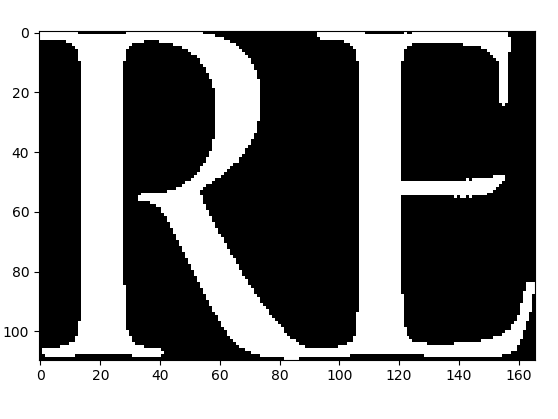
\includegraphics[height=50px]{1.png}			
		\end{figure}
		\begin{figure}[H]			
			\caption[Vizinhança do pixel]
			{Vizinhança do pixel}
			\centering
			\begin{subfigure}[b]{50px}				
				\caption{8-conexa}
				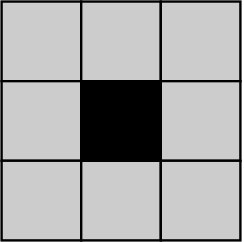
\includegraphics[width=\textwidth]{2.png}
			\end{subfigure}
			~
			\begin{subfigure}[b]{50px}				
				\caption{4-conexa}
				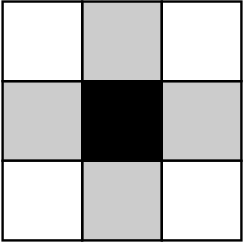
\includegraphics[width=\textwidth]{3.png}
			\end{subfigure}	\\
			{Fonte: \href{https://en.wikipedia.org/wiki/Pixel\_connectivity}{https://en.wikipedia.org/wiki/Pixel\_connectivity}}	
		\end{figure}
			
		Neste trabalho, considera-se a vizinhança 8-conexa. 
	
	\subsection{Superpixels}
		Superpixels agrupam pixels em regiões que possuem algum sentido, geralmente, capturando redundâncias em imagens e reduzindo a complexidade do processamento subsequente. 
		
		Existem muitas formas de gerar superpixels, cada qual com vantagens e desvantagens. Nesta pesquisa, utilizou-se do Simple Linear Itarative Clustering (SLIC), que se baseia no algoritmo de clustering K-means para gerar os superpixels como se fossem clusters, em um espaço onde as dimensões são as coordenadas x,y,z e as cores. Dentre os benefícios do SLIC estão: facilidade de uso, flexibilidade de controle da compacidade e do número de superpixels que são gerados \cite{Achanta:2012}. 
		
		\begin{figure}[H]			
			\caption[Superpixels]
			{Os superpixels calculados pelo SLIC  na região correspondente ao componente conexo da figura 1}
			\centering
			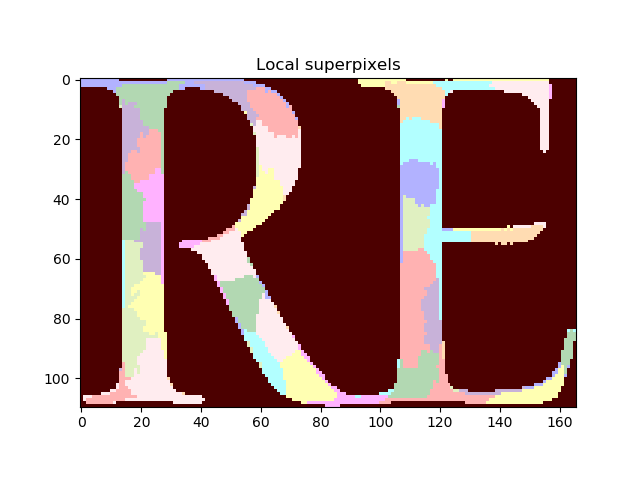
\includegraphics[height=100px]{4.png}			
		\end{figure}
	
	\subsection{Redes Neurais Convolucionais}
		
		Uma Rede Neural regular recebe um vetor de entrada e transforma-o através de camadas ocultas. Cada camada possui seus neurônios, que são conectados atráves conexões que têm um certo peso associado - parâmetro que é aprendido durante o treinamento - a todos os neurônios da camada anterior, mas funcionam de forma independente dentro da camada, por não compartilhar conexões com outros neurônios da mesma camada. Um neurônio calcula uma combinação linear de suas entradas, ponderadas pelos respectivos pesos, e o valor resultante é transformado por uma função não linear, tais como a sigmoide ou ReLU, chamadas de função de ativação. A última camada é chamada de "camada de saída" e geralmente devolve os \textit{scores} de cada classe \cite{Yaser:2012}. 
		
		É importante mencionar que Redes Neurais não funcionam bem para imagens grandes. Por exemplo, para uma imagem de 300x300x3, cada neurõnio na primeira camada oculta terá 270.000 pesos, que é a quantidade pixels na imagem de entrada multiplicada pelas intensidades nos canais R, G e B. 
		
		As Redes Neurais Convolucionais (CNN, na sigla em inglês), por sua vez, pressupõem que a entrada é composta por imagens e, partindo disso, têm uma arquitetura especial para lidar com esse tipo de aprendizado. Para começar, nas CNNs, cada camada de neurônio possui três parâmetros: largura, altura e profundidade. Além disso, os neurônios em cada camada só estão ligados a uma pequena região da camada anterior, ao invés de estarem ligados a todos os anteriores ~\cite{stanford:cnn}. 
		
		\begin{figure}[H]			
			\caption[CNNs x MLP ]
			{MLP x CNN}
			\centering
			\begin{subfigure}[b]{150px}				
				\caption{Rede Neural regular}
				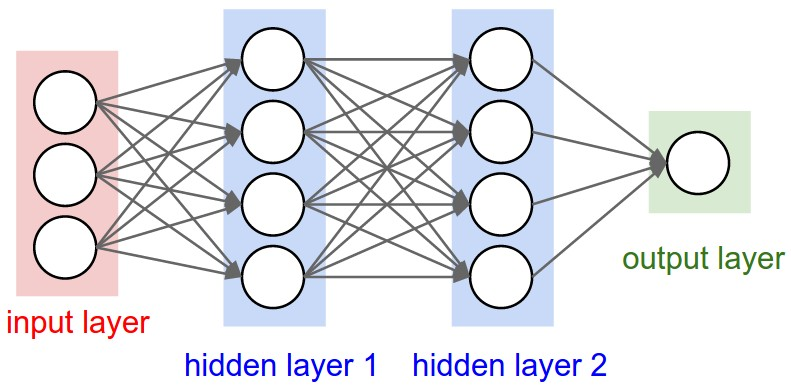
\includegraphics[width=\textwidth]{5.jpeg}
			\end{subfigure}
			\qquad
			\begin{subfigure}[b]{150px}				
				\caption{Rede Neural Convolucional}
				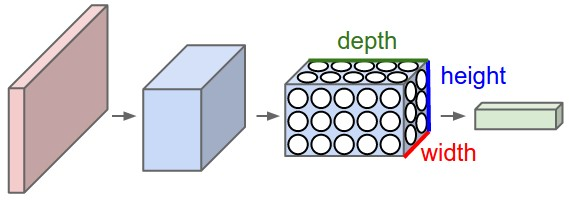
\includegraphics[width=\textwidth]{6.jpeg}
			\end{subfigure}	\\
			{Fonte: \href{http://cs231n.github.io/convolutional-networks/}{http://cs231n.github.io/convolutional-networks/}}	
		\end{figure}
			
		Existem três principais tipos de camada na arquitetura de uma CNN: camada convolucional, camada de \textit{pooling} e camada \textit{fully-connected}. A camada convolucional calcula a saída de neurônios que estão conectados a regiões locais na entrada, cada qual computando um produto escalar entre os seus pesos e a pequena região a qual eles estão conectados. 
		Já a camada de \textit{pooling} vai reescalar a saída da camada convolucional para que ela tenha dimensões menores, por exemplo, de 32x32x12 para 16x16x12. Por fim, a camada \textit{fully-connected} (que basicamente é uma Rede Neural regular) computa os \textit{scores} das classes, resultando num tensor de dimensões 1x1xn, onde n é o número de classes. 
		
		\begin{figure}[H]			
			\caption[Arquitetura da CNN]
			{Arquitetura da CNN, onde \textit{subsamplings} referem-se às camadas de pooling mencionadas anteriormente}
			\centering
			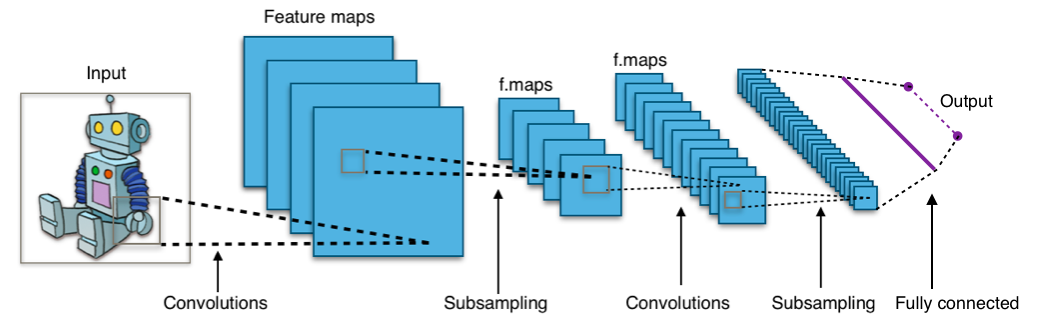
\includegraphics[height=80px]{8.png}	\\
			{Fonte: \href{https://en.wikipedia.org/wiki/Convolutional\_neural\_network}{https://en.wikipedia.org/wiki/Convolutional\_neural\_network}}		
		\end{figure}
		
	
	\subsection{Métricas}
	
		Uma matriz de confusão para problemas de classificação binária (positivo x negativo) é uma tabela que permite a visualização do desempenho de um algoritmo, através da contagem dos seguintes valores ~\cite{wiki:confusion}: 
		
		\begin{itemize}
			\item verdadeiros positivos (TP): quando um exemplo positivo é corretamente classificado como positivo.
			\item verdadeiros negativos (TN): quando um exemplo negativo é corretamente classificado como negativo.
			\item falsos positivos (FP): quando um exemplo negativo é erroneamente classificado como positivo.
			\item falsos negativos (FN): quando um exemplo positivo é erroneamente classificado como negativo. 
		\end{itemize}		
		
		\begin{longtable}[c]{@{}cc
				>{\columncolor[HTML]{9FA8DA}}c 
				>{\columncolor[HTML]{9FA8DA}}c @{}}	
			\caption[Matriz de confusão]{Matriz de confusão} \\		
			\multicolumn{2}{c}{}                                                                          & \multicolumn{2}{c}{\cellcolor[HTML]{9FA8DA}Valores verdadeiros}                \\
			\multicolumn{2}{c}{\multirow{-2}{*}{}}                                                        & Positivo                                          & Negativo                   \\
			\endfirsthead
			%
			\endhead
			%
			\cellcolor[HTML]{FFF59D}                                   & \cellcolor[HTML]{FFF59D}Positivo & \cellcolor[HTML]{A5D6A7}{\color[HTML]{000000} TP} & \cellcolor[HTML]{EF9A9A}FP \\
			\multirow{-2}{*}{\cellcolor[HTML]{FFF59D}Valores preditos} & \cellcolor[HTML]{FFF59D}Negativo & \cellcolor[HTML]{EF9A9A}FN                        & \cellcolor[HTML]{A5D6A7}TN
		\end{longtable}
		
		Dessas contagens, obtém-se outras três métricas: acurácia, precisão e \textit{recall}. Considera-se que a acurácia é uma descrição dos erros sistemáticos. As predições de um algoritmo são acuradas se elas estão próximas dos valores verdadeiros do rótulo de cada exemplo ~\cite{wiki:acc}.
		
		\begin{equation}
			accuracy = \frac{TP+FN}{TP+TN+FP+FN}
			\nonumber
		\end{equation}
		
		A precisão, por sua vez, revela quantos dos exemplos classificados como positivos são realmente positivos ~\cite{wiki:pre}. 
		
		\begin{equation}
			precision = \frac{TP}{TP+FP}
		\nonumber
		\end{equation}
		
		Por fim, o \textit{recall} (também chamado de sensibilidade) mede a proporção de quantos positivos foram corretamenete classificados dentro do conjunto de todos os positivos verdadeiros ~\cite{wiki:pre}. 
		
		\begin{equation}
			recall = \frac{TP}{TP+FN}
		\nonumber
		\end{equation}	
	
	\section{Método}
	
		A transformação considerada neste trabalho é a segmentação de
		texto em imagens de páginas de documentos. Um exemplo de
		imagem de entrada e de saída esperada é mostrado na figura 6. (a). Trata-se de um problema de classificação binária, no qual cada pixel na imagem de saída terá valor 1 caso corresponda a um pixel de texto e valor 0 em caso contrário.
	
		Como exemplos, utilizaram-se imagens de entrada em formato JPG e, como rótulos, imagens PNG, nas quais cada pixel tinha valor 0 (não-texto) ou 1 (texto). 
		
		\begin{figure}[H]			
			\caption[Conjunto de dados]
			{Conjunto de dados}
			\centering
			\begin{subfigure}[b]{150px}				
				\caption{Imagem de entrada}
				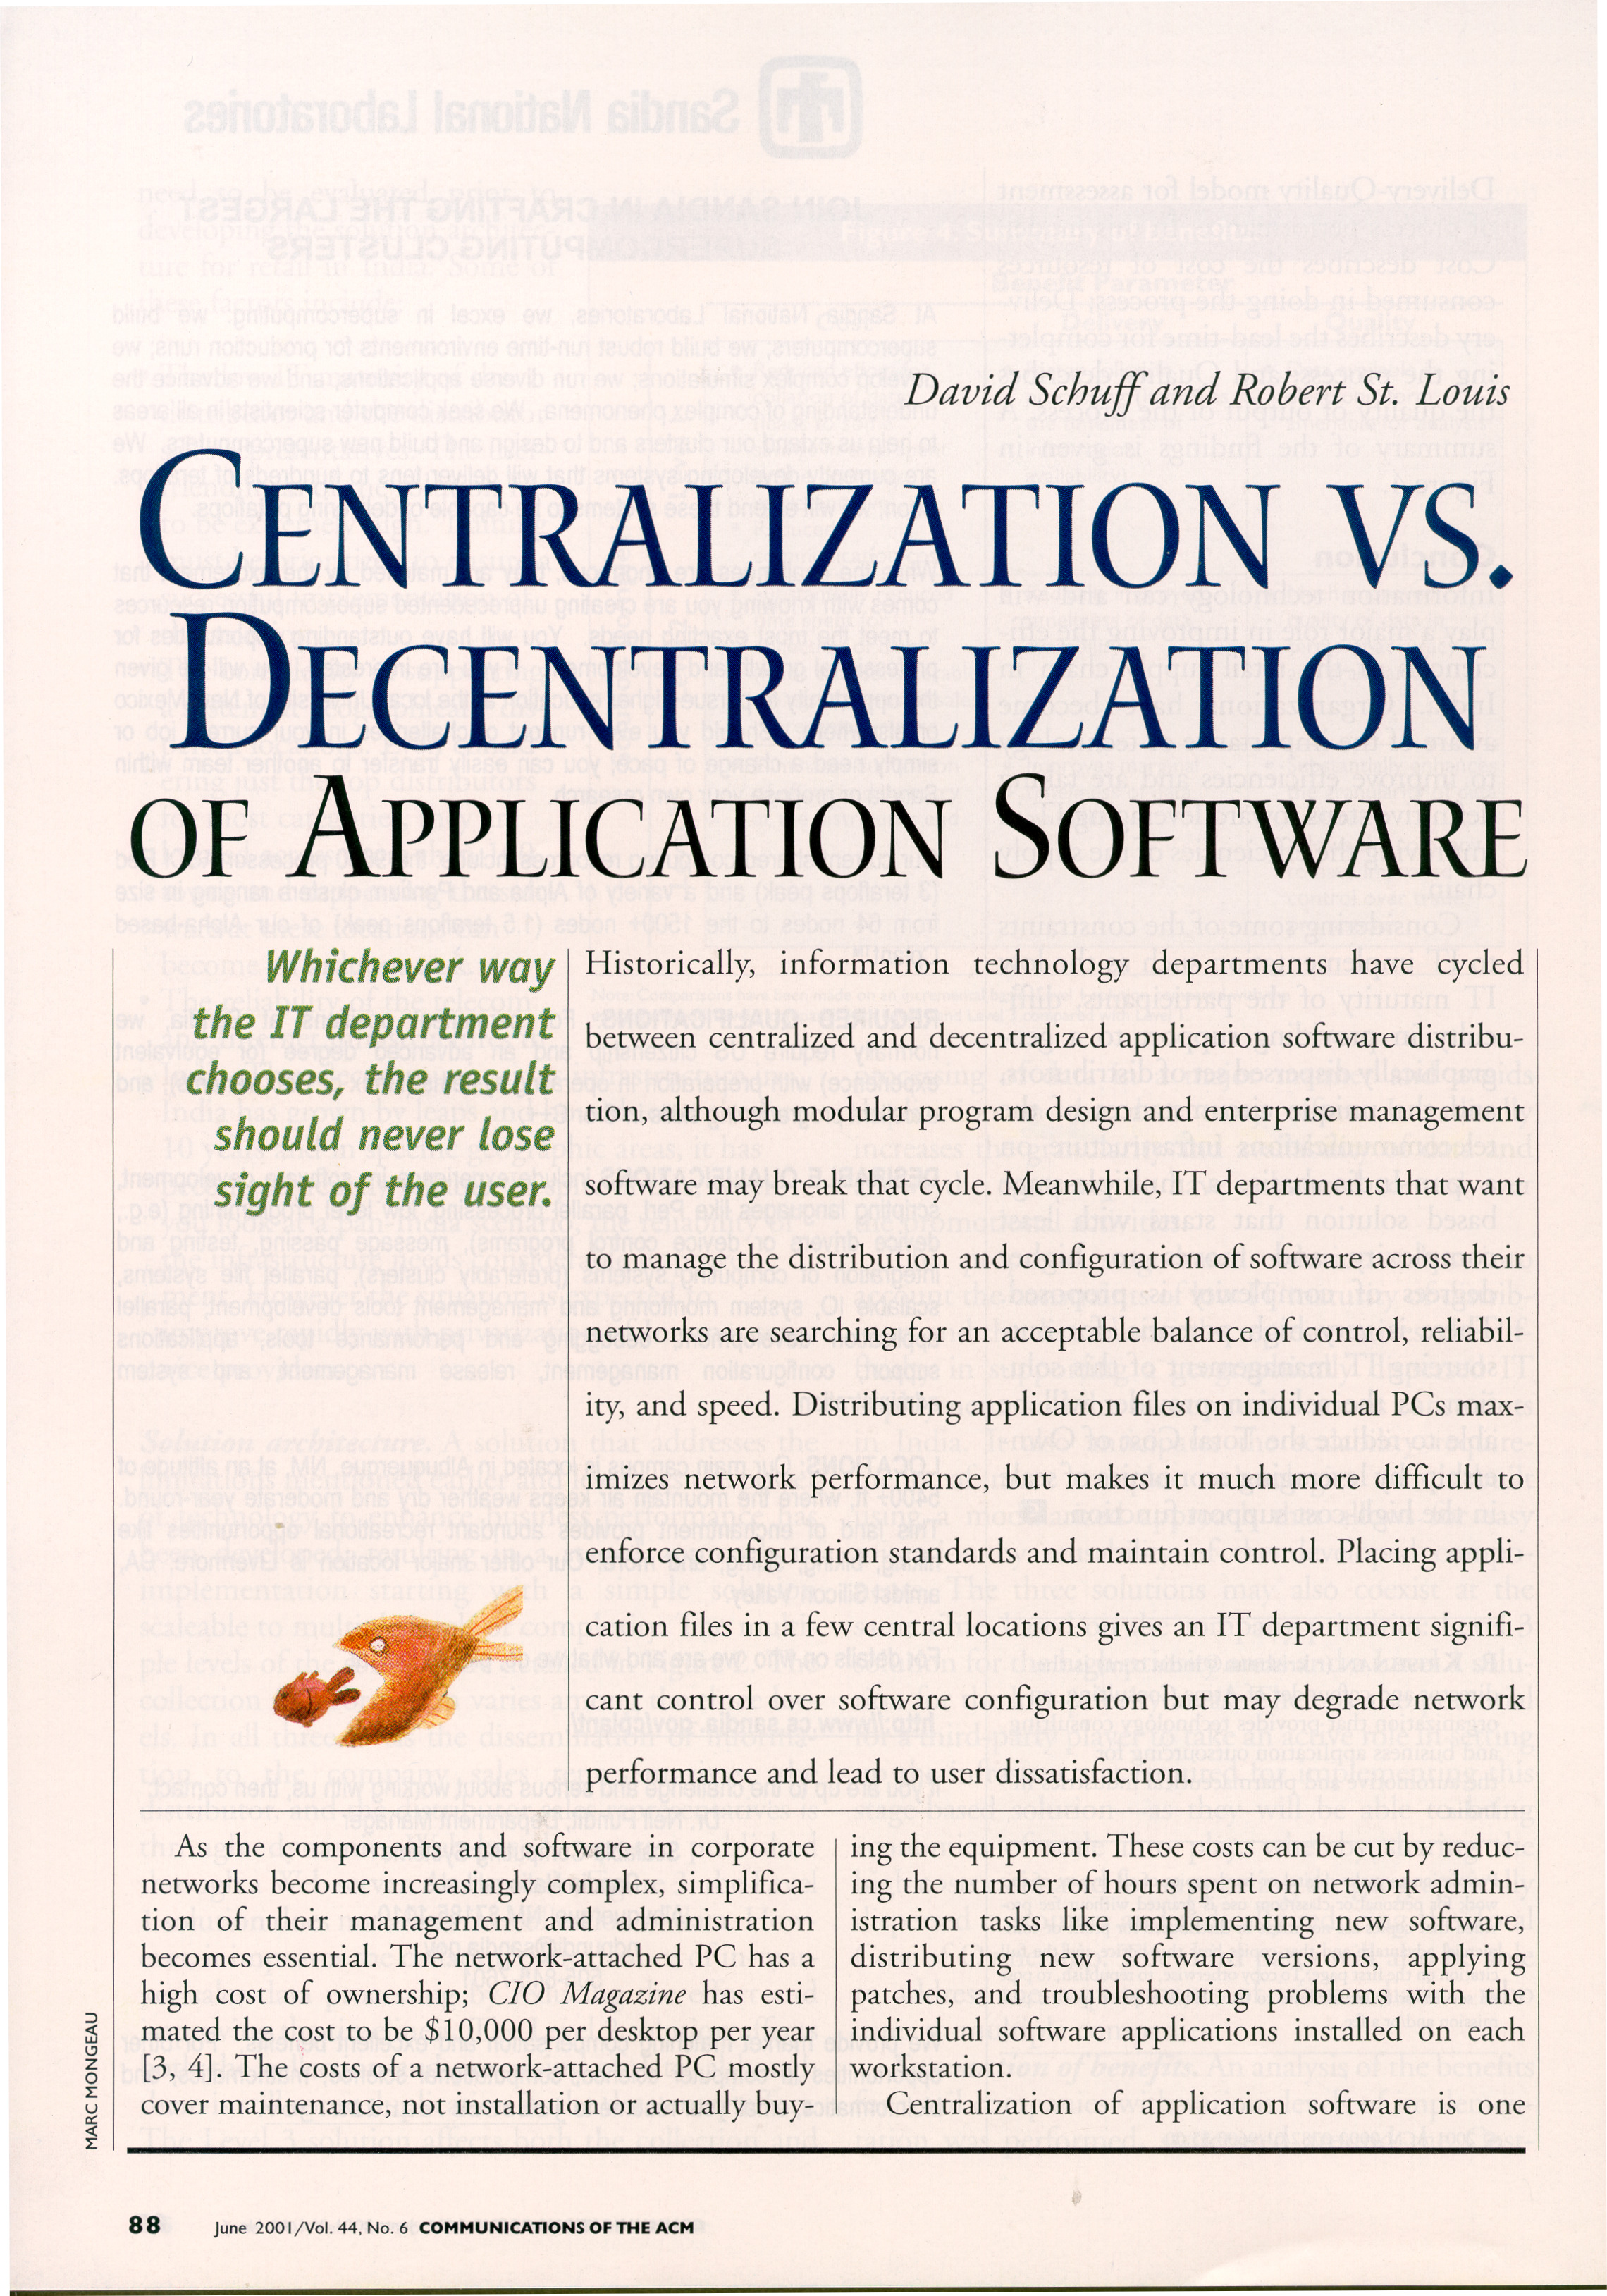
\includegraphics[width=\textwidth]{9.jpg}
			\end{subfigure}
			\qquad
			\begin{subfigure}[b]{150px}				
				\caption{Rótulo}
				
\includegraphics[width=\textwidth]{10.png}
			\end{subfigure}	\\	
		\end{figure}
		
		Primeiramente, transformou-se a imagem RGB em uma versão em tons de cinza. Em seguida, utilizou-se o método de Otsu para binarizar a imagem cinza. Para segmentar essas imagens de exemplos em componentes conexos, utilizou-se a função "label". Todas as funções que foram usadas para fazer os passos anterior estão disponíveis na biblioteca scikit-image \footnote{\url{https://scikit-image.org/}}, codificada em Python. Já para o cômputo dos superpixels, calculou-se esses elementos somente sobre os componentes conexos selecionados (aqueles que tinham área acima de um determinado valor). Para isso, utilizou-se a função "slic", disponível também na bilioteca scikit-image. 
		
		\begin{figure}[H]			
			\caption[Microrregiões]
			{Microrregiões}
			\centering
			\begin{subfigure}[b]{150px}				
				\caption{Componente conexo}
				
\includegraphics[width=\textwidth]{11.png}
			\end{subfigure}
			\qquad
			\begin{subfigure}[b]{150px}				
				\caption{Superpixels}
				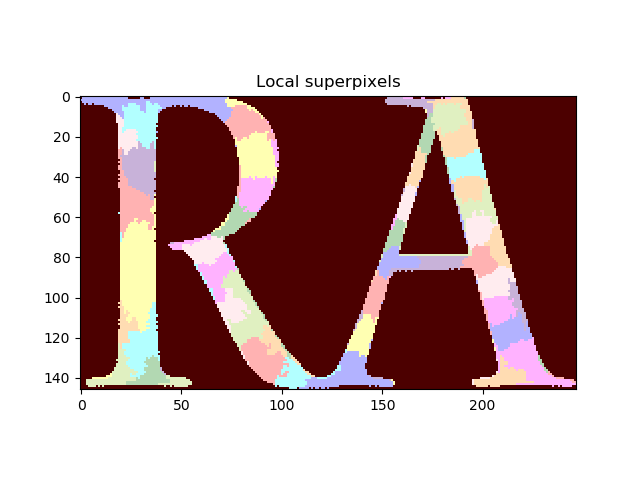
\includegraphics[width=\textwidth]{12.png}
			\end{subfigure}	\\	
		\end{figure}
	
		Três pipelines foram utilizados, um para cada uma das granularidades investigadas neste trabalho: sobre pixels, sobre superpixels e sobre componentes conexos. 
		
		A nível de pixels, quanto ao conjunto de treino, basicamente, para cada unidade atômica da imagem, gera-se um janela de dimensões 21x21 centrada no pixel em questão. Com os \textit{patches} forma-se um \textit{array} de dimensões (n, 21, 21, 3), onde n é o número de \textit{patches} extraídos da imagem. Para cada um desses \textit{patches}, há um rótulo, que é a classificação do pixel central (0 ou 1). 
		
		\begin{figure}[H]			
			\caption[Pipeline da predição sobre os pixels]{Pipeline da predição sobre os pixels}
			\centering
			
\includegraphics[width=400px]{13.png}			
		\end{figure}
		
		No caso das microrregiões (que compreendem os superpixels e os componentes conexos), o \textit{pipeline} funciona de maneira similar, mas com algumas etapas adicionais. Primeiramente, calcula-se as microrregiões. Então, para cada componente conexo ou superpixel, gera-se um \textit{patch} em volta do elemento em questão de tal maneira que, quando redimensionado para dimensões 41x41x3, a microrregião fique ao centro com tamanho 9x9x3. A partir da obtenção do \textit{patch}, o processo é idêntico ao descrito anteriormente. Vale ressaltar que, nesse caso, cada \textit{patch}	tem o rótulo da respectiva microrregião. Para os casos em que a mesma microrregião têm dois rótulos, considera-se o que está mais frequente dentro desse elemento. 
		
		\begin{figure}[H]			
			\caption[Pipeline da predição sobre microrregiões]{Pipeline da predição sobre microrregiões}
			\centering
			
\includegraphics[width=400px]{14.png}			
		\end{figure}
		
		Para obter uma imagem de saída, faz-se procedimento similar: o algoritmo faz a predição para cada \textit{patch} extraído da imagem de teste. Por fim, pinta-se o elemento da saída (pixel, componente conexo ou superpixel) com o valor da predição de seu respectivo \textit{patch}.
		
		As atividades realizadas, bem como a quantidade de horas semanais despendidas durante o primeiro semestre de 2019 podem ser conferidas no anexo \ref{appendix:atividades}. Essa mesma informação pode ser encontrada com maior detalhadamento, incluindo a quantidade de horas por atividades e provas da execução da mesma (\textit{commits}, resumo, e-mails) no endereço \href{https://github.com/robonauta/IC/tree/master/acompanhamento}{https://github.com/robonauta/IC/tree/m\\as ter/acompanhamento}.
		
	\section{Resultados}
	
		Originalmente, as imagens do conjunto de dados tinham dimensões 2280x3257x3. Ao seguir o pipeline proposto, essas imagens resultavam num conjunto de 7.425.960 de \textit{patches}, no caso dos pixels - número computacionalmente inviável. Então, para fazer uma comparação justa entre as três granularidades, reduziram-se essas imagens para 250x357x3. Além disso, utilizou-se apenas uma imagem para treinamento e outra diferente para os testes. A justificativa é a limitação de espaço na memória. Os resultados para essa configuração podem ser vistos na tabela abaixo. 
		
		\begin{longtable}[c]{@{}cccc@{}}
			\caption[Resultados da configuração I]{Resultados da para imagens de dimensões 250x357x3} \\
			\toprule
			\multicolumn{4}{c}{Configuração I}                                                        \\* \midrule
			& Pixels & Componentes conexos & Superpixels \\* \midrule
			\endfirsthead
			%
			\endhead
			%
			\bottomrule
			\endfoot
			%
			\endlastfoot
			%
			Número de patches                         & 86500  & 135                 & 277         \\
			Tempo para extração de patches (segundos) & 1,7740 & 0,2104              & 2,9262      \\
			Acurácia                                  & 0,9183 & 0,9832              & 0,9763      \\
			Precisão                                  & 0,8150 & 0,9857              & 0,9816      \\
			Recall                                    & 0,7692 & 0,9974              & 0,9940      \\* \bottomrule
		\end{longtable}
	
	Em seguida, houve a tentativa de treinar e testar as CNNs nas imagens com as suas dimensões originais. Para issou, utilizaram-se 6 imagens de treino e 4 imagens para teste, todas com dimensões próximas de 2280x3257x3. Os resultados estão na tabela abaixo.
	
	\begin{longtable}[c]{@{}cccc@{}}		
		\caption[Resultados da configuração II]{Resultados da para imagens de dimensões 2280x3257x3} \\
		\toprule
		\multicolumn{4}{c}{Configuração II}                                                        \\* \midrule
		\endfirsthead
		%
		\endhead
		%
		Métrica                                   & Pixels      & Componentes conexos & Superpixels \\* \midrule
		Número de patches                         & MemoryError & 3322                & 16395       \\* 
		Tempo para extração de patches (segundos) & MemoryError & 5,4418              & 62,4901     \\* 
		Acurácia                                  & MemoryError & 0,9959              & 0,9908      \\* 
		Precisão                                  & MemoryError & 0,9973              & 0,9969      \\* 
		Recall                                    & MemoryError & 0,9984              & 0,9889      \\* \bottomrule
	\end{longtable}
		
	\section{Discussão}	
	
	Como pode-se perceber, o número de \textit{patches} foi reduzido em aproximadamente 99,84\% no caso dos componentes conexos (CCs) e em 99,67\% no caso dos superpixels (SPs). Isso é bastante importante para que seja possível aumentar os conjuntos de treinamento e teste, bem como, reduzir a complexidade computacional de todo o processo. 
	
	Nota-se que o desempenho da classificação de microrregiões foi superior ao da classificação pontual, sendo os CCs a granularidade que mais se destaca na acurácia, apesar da pequena diferença para a rotulação de superpixels. 
	
	Em contrapartida, chega-se a perder um certo tempo para calcular as microrregiões, sendo o cálculo dos superpixels, através do SLIC, o mais demorado. No entanto, como a quantidade de pixels chega com muita frequência aos milhões, pode acontecer do tempo para o cômputo dos \textit{patches} de CCs ser menor que o tempo para o cálculo dos patches de cada um dos pixels. 
	
	Outro ponto relevante a ser mencionado é a distorção que as métricas podem causar. Os componentes conexos, apesar de terem a maior acurácia, têm o seguinte problema no treinamento: como as letras (rotuladas como texto) geram a esmagadora maioria dos \textit{patches}, a CNN acaba aprendendo a classificar melhor os elementos que são texto, em detrimento daqueles que não são. Por essa razão, muitas imagens dispostas entre o texto das revistas acabam sendo classificadas como "texto" (apenas pela razão de formarem um componente conexo). 
	
	\begin{figure}[H]			
		\caption[Imagens de entrada e saída]
		{Algumas imagens da folha da revista foram classificadas como "texto"}
		\centering
		\begin{subfigure}[b]{90px}				
			\caption{Imagem de entrada}
			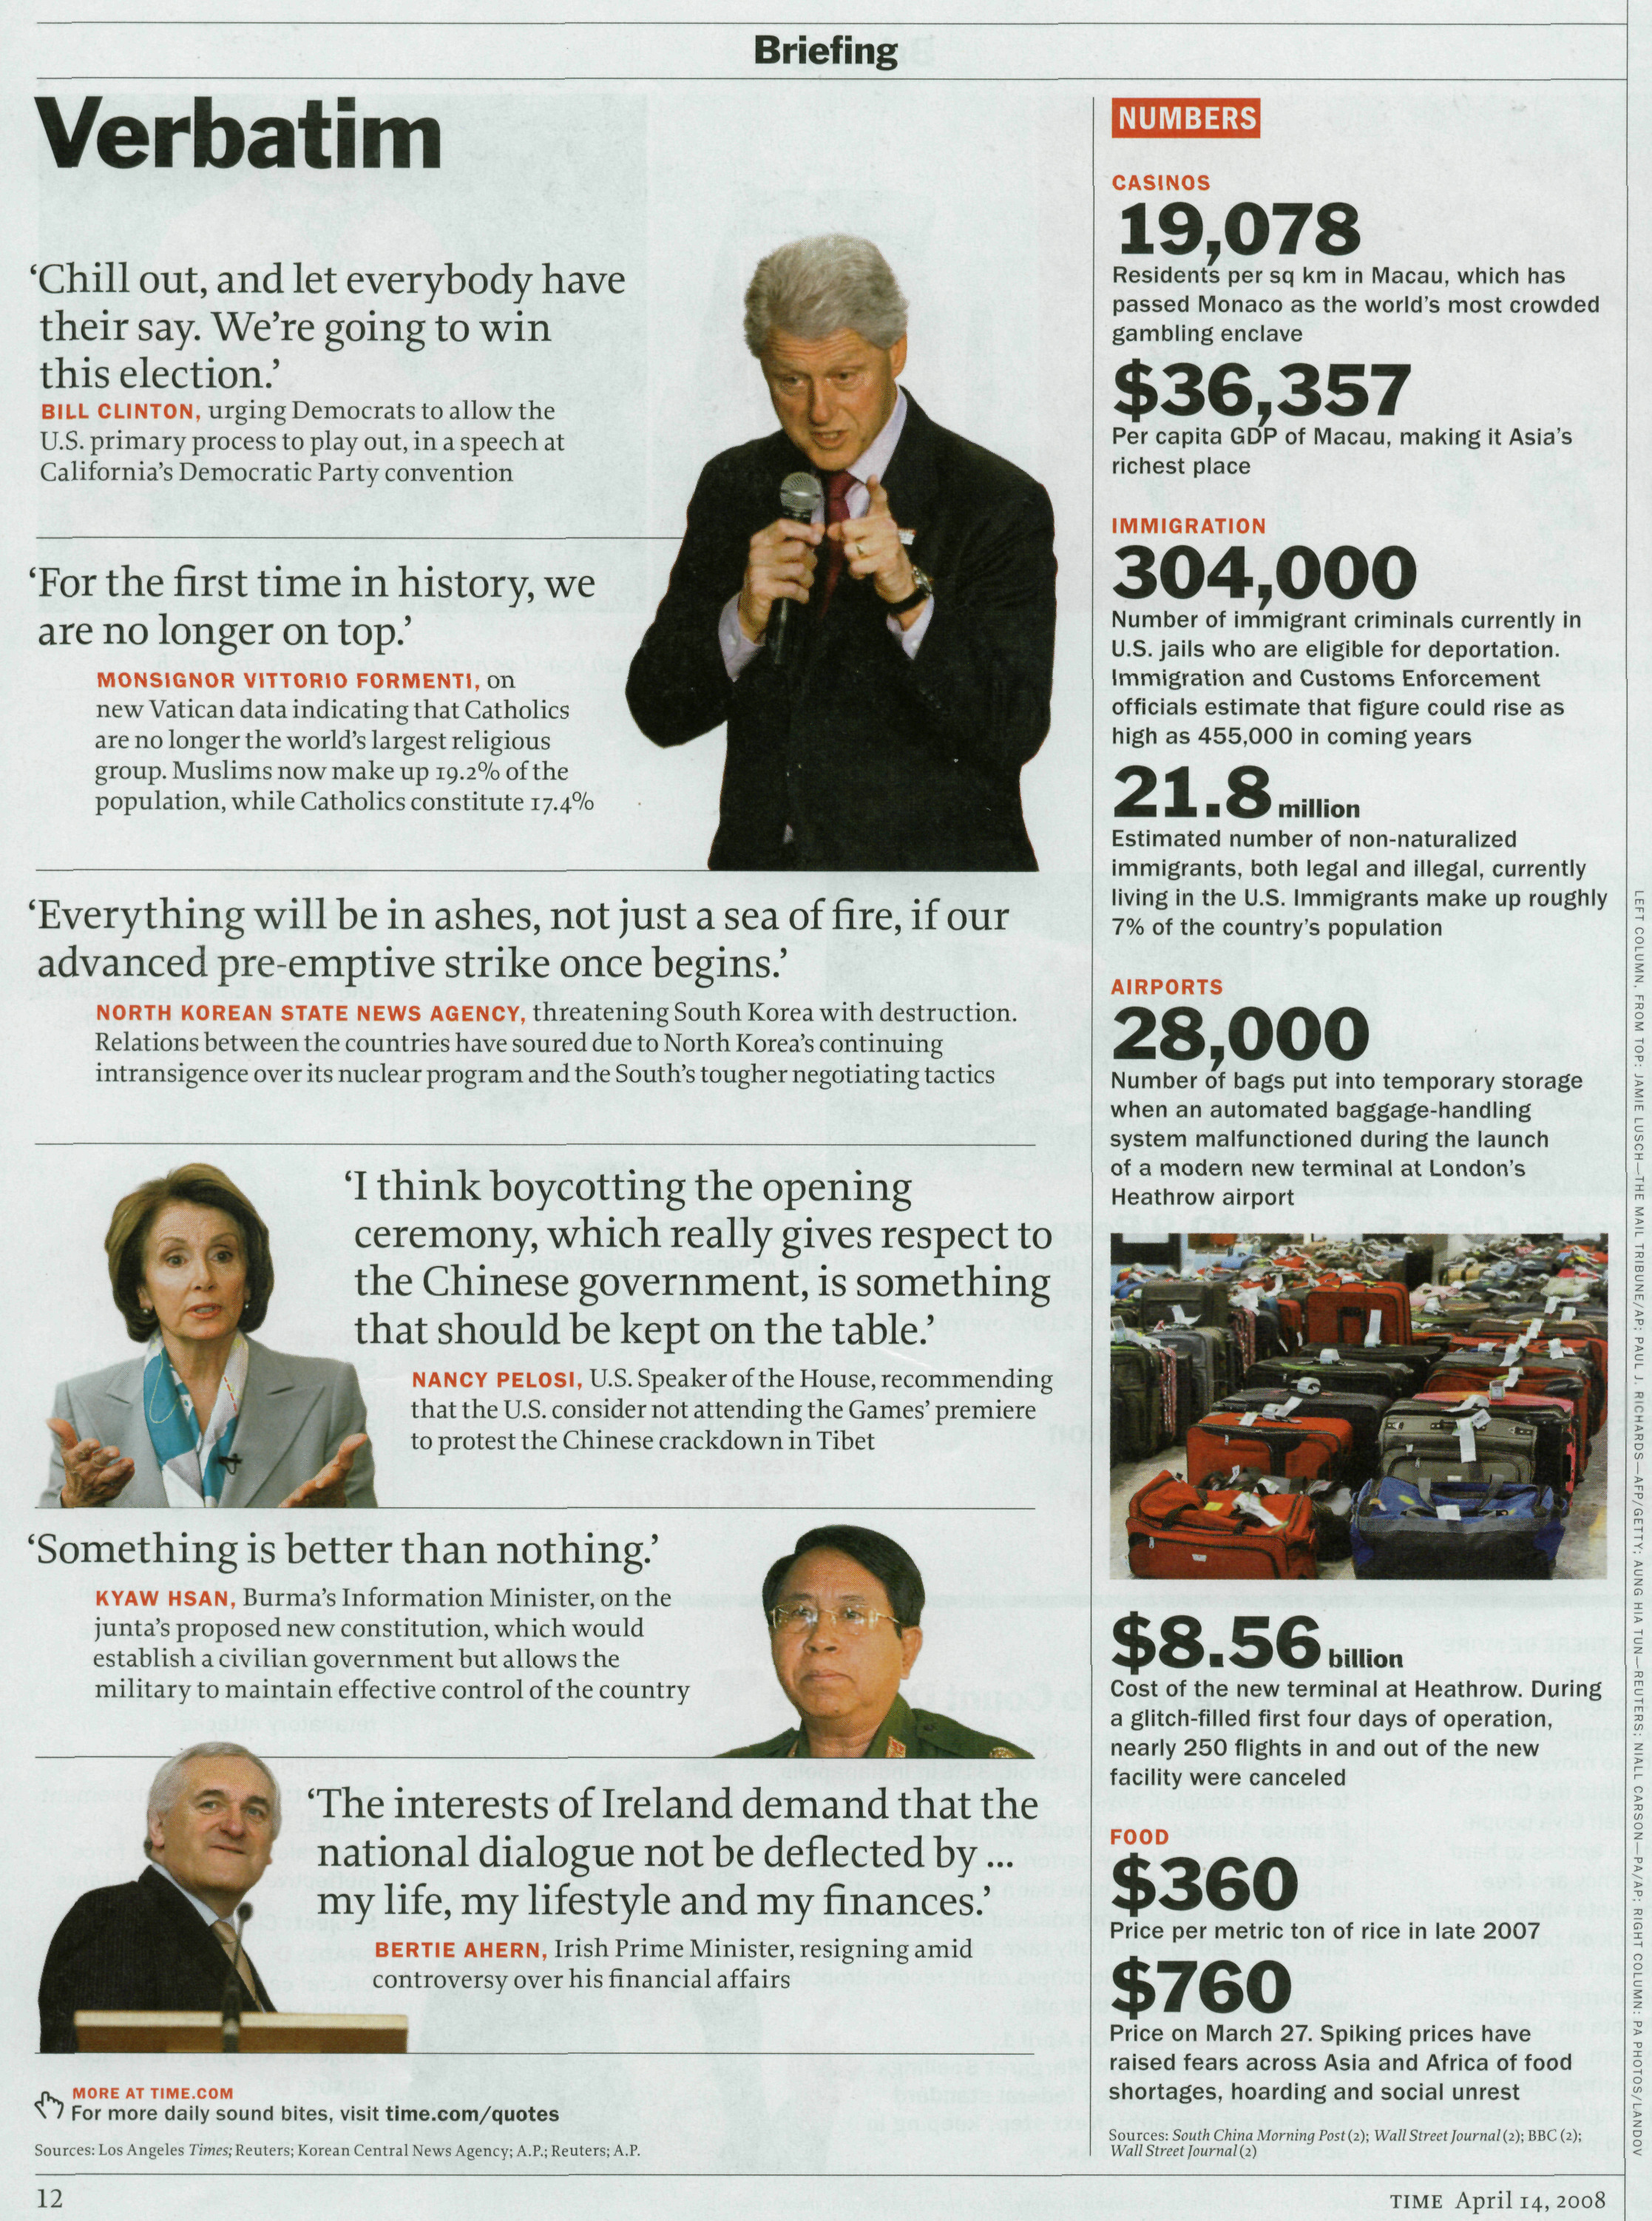
\includegraphics[width=\textwidth]{16.jpg}
		\end{subfigure}
		\qquad
		\begin{subfigure}[b]{90px}				
			\caption{Ground-truth}
			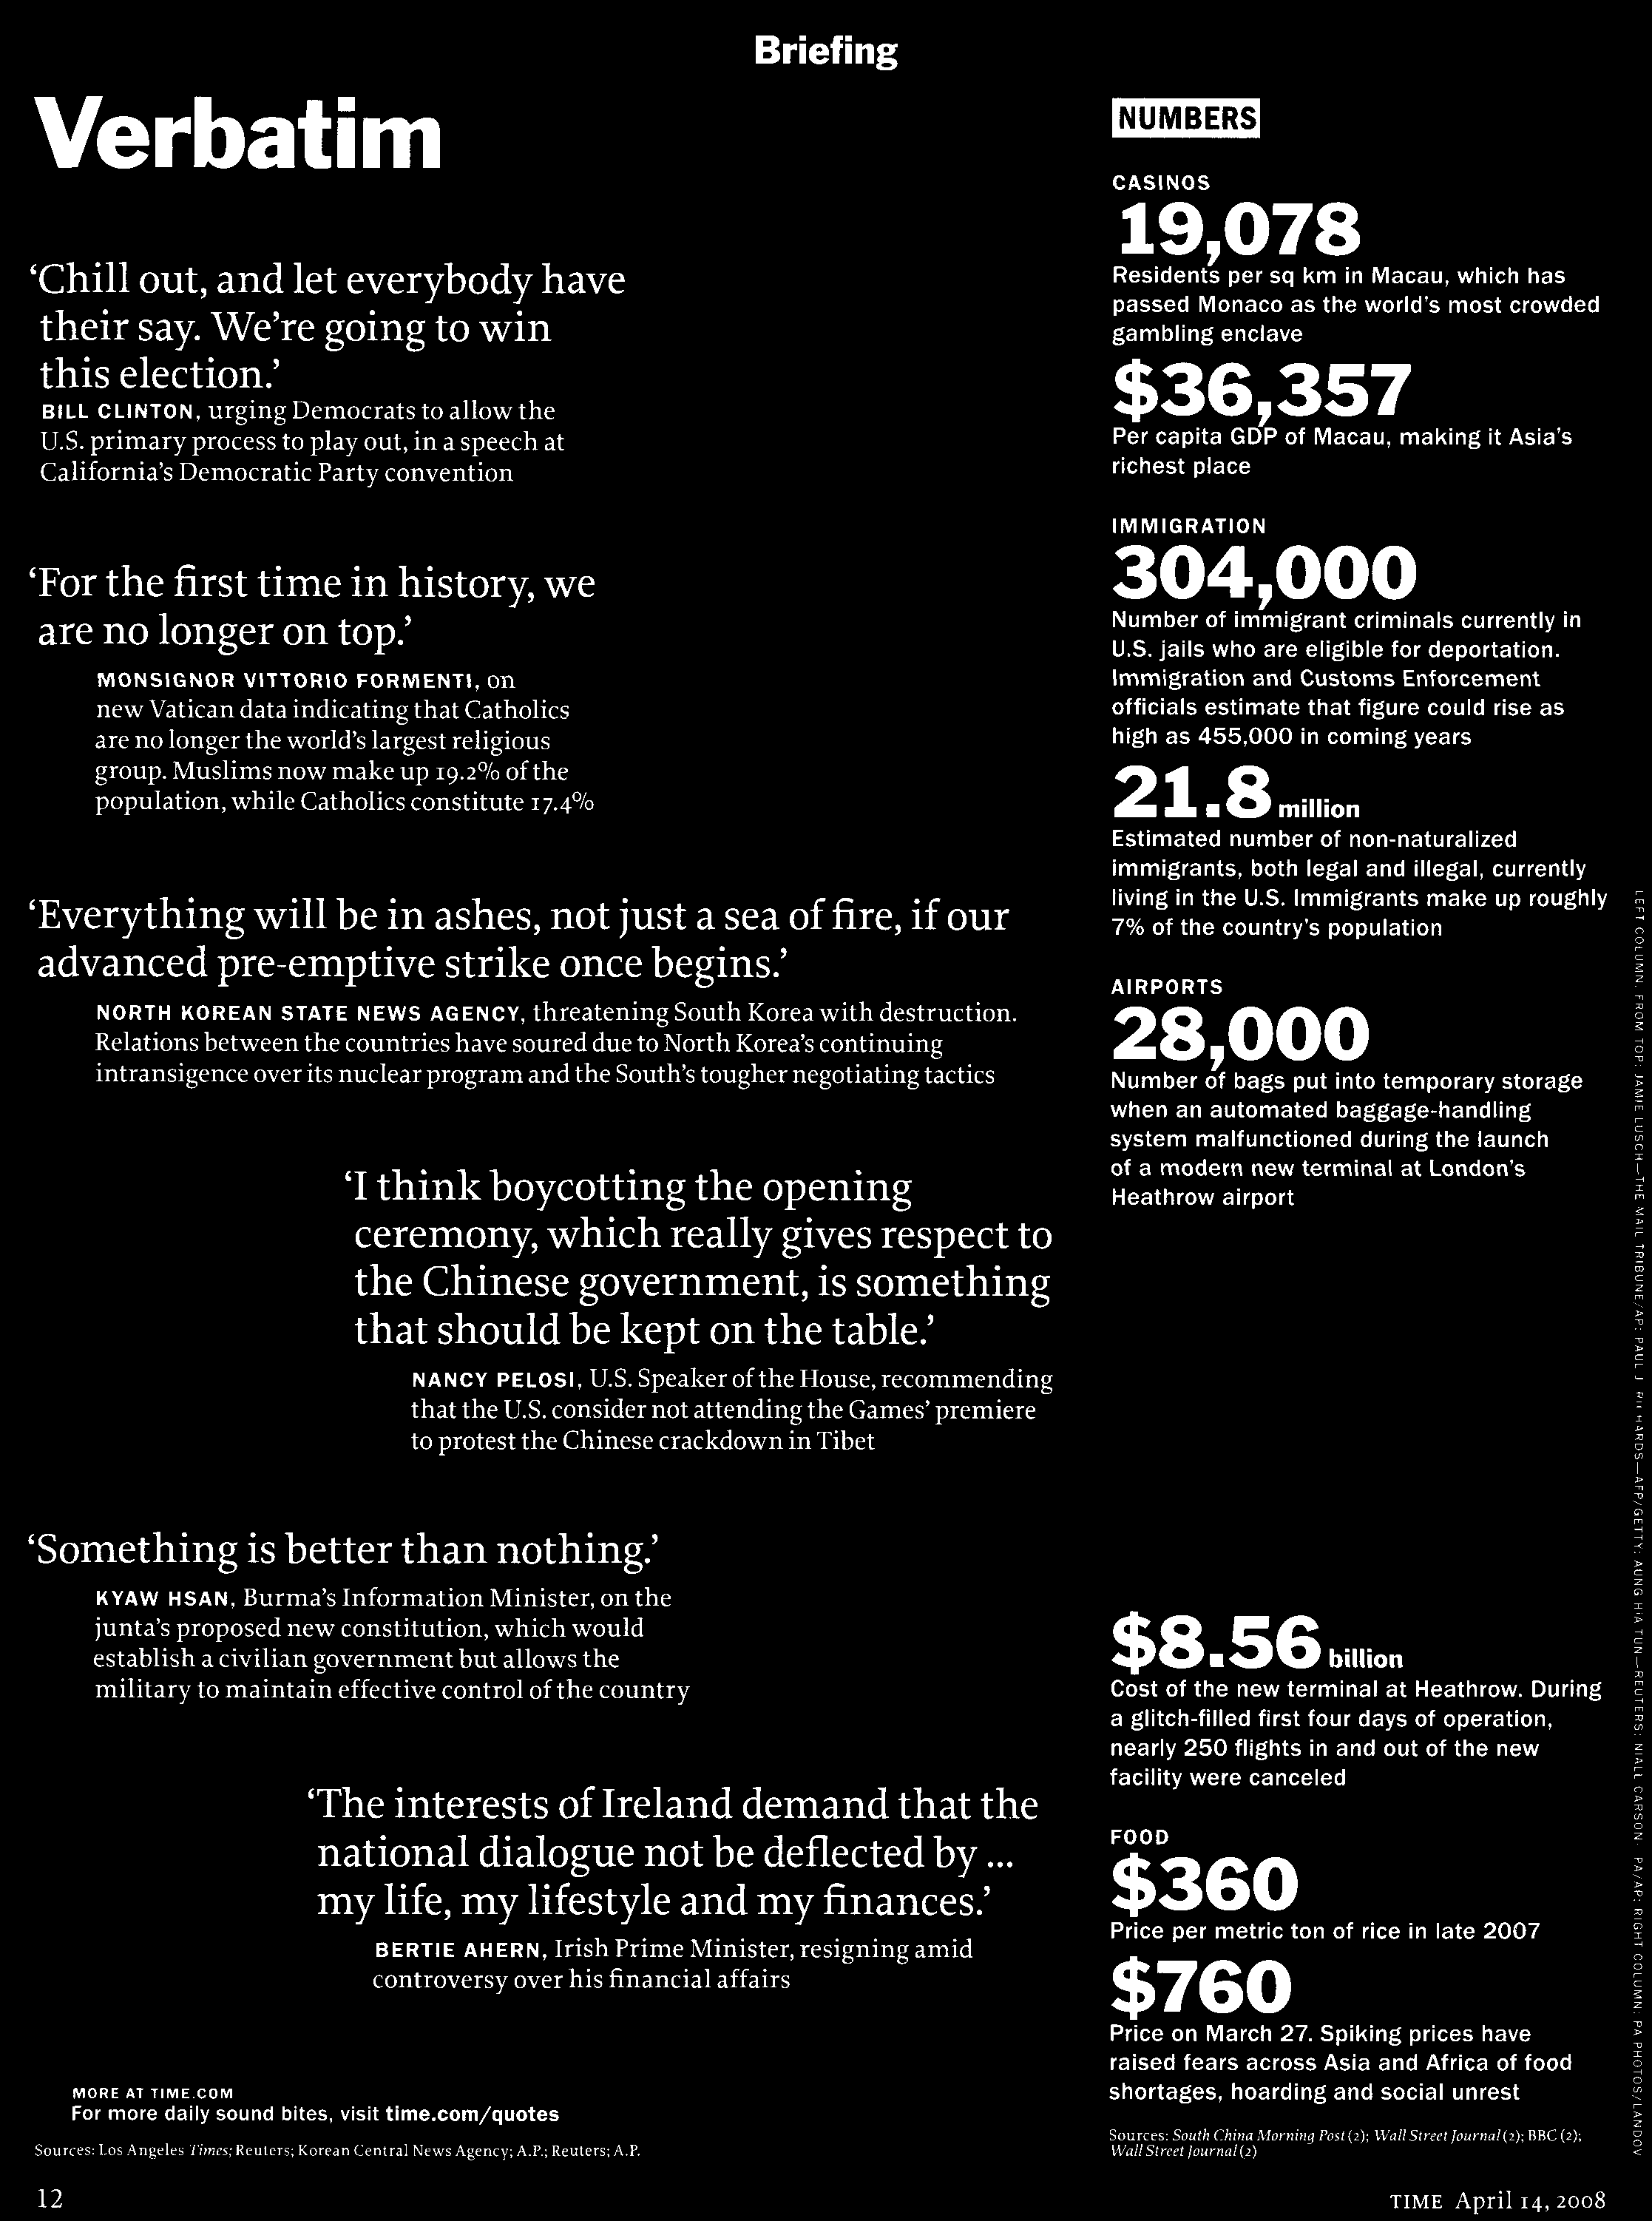
\includegraphics[width=\textwidth]{17.png}
		\end{subfigure}	
		\qquad
		\begin{subfigure}[b]{90px}				
			\caption{Imagem de saída}
			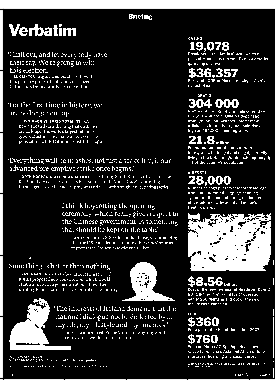
\includegraphics[width=\textwidth]{15.png}
		\end{subfigure}
	\end{figure}
	
	Dessa forma, para os próximos meses de vigência dessa Iniciação Científica, buscar-se-á investigar como certos parâmetros como o tamanho do \textit{patch} e a arquitetura da rede podem variar e melhorar os resultados obtidos. Além disso, são almejadas formas de se contornar os erros de memória ao aumentar os conjuntos de treinamento e teste, bem como formas de diminuir a disparidade entre o número de exemplos de cada classe no caso dos componentes conexos. 
	
	\newpage
	
	\bibliographystyle{apalike}
	\bibliography{refs}
	
	\newpage
	
	\begin{appendices}		
		{\setlength{\parindent}{0cm}
		\section{Atividades realizadas}
			\label{appendix:atividades}
			\textbf{Semana de 25/02 a 03/03} 
			\begin{itemize}
				\item Reunião semanal com o grupo de pesquisa
			\end{itemize}			
			Horas gastas: 2h \\
			
			\textbf{Semana de 04/03 a 10/03}
			\begin{itemize}
				\item Reunião semanal com o grupo de pesquisa 
			\end{itemize}
			Horas gastas: 2h \\
			
			\textbf{Semana de 11/03 a 17/03}
			\begin{itemize}	
				\item Confecção de apresentação do projeto para MAC0215
			\end{itemize}			 
			Horas gastas: 7h \\
			
			\textbf{Semana de 18/03 a 24/03}
			\begin{itemize}
				\item Reunião semanal com o grupo de pesquisa 
				\item Leitura do Módulo 0 - Preparation do curso CS231n
			\end{itemize}
			Horas gastas: 7h \\
			
			\textbf{Semana de 25/03 a 31/03} \\
			Horas gastas: 0h \\
			
			\textbf{Semana de 01/04 a 07/03}
			\begin{itemize}
				\item Leitura e resumo do Módulo 1 - Image Classification 
				\item Reunião semanal com o grupo de pesquisa 
			\end{itemize}
			Horas gastas: 5h \\
			
			\textbf{Semana de 08/04 a 14/04}
			\begin{itemize}
				\item Oficina de Convnets no Keras com a orientadora 			
			\end{itemize}
			Horas gastas: 2h \\
			
			\textbf{Semana de 15/04 a 21/04} \\
			Horas gastas: 0h \\
			
			\textbf{Semana de 22/04 a 28/04}
			\begin{itemize}
				\item Leitura e resumo do Módulo 1 - Linear Classification 
				\item Leitura e resumo do Módulo 1 - Optimization 
				\item Leitura e resumo do Módulo 1 - Backpropagation 
				\item Leitura e resumo do Módulo 1 - Neural Networks Part 1 
				\item Leitura e resumo do Módulo 1 - Neural Networks Part 2 
			\end{itemize}
			Horas gastas: 9h \\
			
			\textbf{Semana de 29/04 a 05/05}
			\begin{itemize}
				\item Leitura e resumo do Módulo 1 - Neural Networks Part 3 
				\item Leitura do Módulo 1 - Putting it together
				\item Leitura e resumo do Módulo 2 - Convolutional Neural Networks 
				\item Leitura e resumo do Módulo 2 - Understanding and Visualizing Convolutional Neural Networks 
				\item Leitura e resumo do Módulo 2 - Transfer Learning 
				\item Leitura dos capítulos 2, 3, 4 e 5 do tutorial de Deep Learning com Keras
				\item Análise dos códigos de classificadores já desenvolvidos pelo grupo de pesquisa 
				\item Reunião semanal com o grupo de pesquisa 			
			\end{itemize}
			Horas gastas: 14h \\
			
			\textbf{Semana de 06/05 a 12/05}
			\begin{itemize}
				\item Reunião semanal com o grupo de pesquisa 			
			\end{itemize}
			Horas gastas: 2h \\
			
			\textbf{Semana de 13/05 a 19/05}
			\begin{itemize}
				\item Programação de programa que extrai patches das imagens 				
			\end{itemize}
			Horas gastas: 10h \\
			
			\textbf{Semana de 20/05 a 26/05}
			\begin{itemize}
				\item Ajustes no algoritmo que extrai patches 
				\item Reunião semanal com o grupo de pesquisa				
			\end{itemize}
			Horas gastas: 4h \\
			
			\textbf{Semana de 27/05 a 02/06}
			\begin{itemize}
				\item Transformação do "patch extractor" para um organizador de dataset (que devolve dados no formato (features, labels)) 
				\item Correção para que os patches da imagem (features) sejam RGB 	
			\end{itemize}
			Horas gastas: 8h \\
			
			\textbf{Semana de 03/06 a 09/06}
			\begin{itemize}
				\item Reunião semanal com o grupo de pesquisa 
				\item Construção de uma rede neural convolucional para treinamento a nível de componentes conexos 
				\item Construção de um "patch extractor" para cada píxel da imagem
				\item Construção de uma rede neural convolucional para treinamento a nível de pixels 			
			\end{itemize}
			Horas gastas: 31h \\
			
			\textbf{Semana de 10/06 a 16/06}
			\begin{itemize}
				\item Construção de um "patch extractor" para cada superpíxel da imagem
				\item Construção de uma rede neural convolucional para treinamento a nível de superpixels 			
			\end{itemize}
			Horas gastas: 7h \\
			
			\textbf{Semana de 17/06 a 23/06}
			\begin{itemize}
				\item Definição e cálculo das métricas de desempenhos das ConvNets para cada granularidade 
				\item Elaboração do pôster 			
			\end{itemize}
			Horas gastas: 15h \\
			
			\textbf{Semana de 24/06 a 30/06}
			\begin{itemize}
				\item Elaboração do relatório final			
			\end{itemize}
			Horas gastas: 15h \\ 
			
			TOTAL DE HORAS GASTAS: 140h
		}
	\end{appendices}
	
\end{document}
